\documentclass{beamer}

\usepackage[utf8]{inputenc}
\usepackage{lmodern}
\usepackage{amsmath}
\usepackage{amsfonts}
\usepackage{amssymb}
\usepackage{bm}
\usepackage{graphicx}
\usepackage{subfigure}
%\usepackage{subcaption}
\usepackage{tikz}
\usepackage{xcolor}
\usepackage{booktabs}
\usepackage{multirow}
\usepackage{color}
\usepackage{colortbl}
\usepackage{cancel}
\usepackage{multimedia}
\usepackage{bibentry} % Enables the command \nobibliography

%\includeonlyframes{f1}

\graphicspath{{./figures/}}

\usetheme{Berlin}
\usecolortheme{beaver}
% //=== The folowing lines are to get rid of navigation bullets
\makeatletter
\setbeamertemplate{headline}
{%
	\begin{beamercolorbox}[colsep=1.5pt]{upper separation line head}
	\end{beamercolorbox}
	\begin{beamercolorbox}{section in head/foot}
		\vskip2pt\insertsectionnavigationhorizontal{\paperwidth}{}{}\vskip2pt
	\end{beamercolorbox}%
	\ifbeamer@theme@subsection%
	\begin{beamercolorbox}[colsep=1.5pt]{middle separation line head}
	\end{beamercolorbox}
	\begin{beamercolorbox}[ht=2.5ex,dp=1.125ex,%
		leftskip=.3cm,rightskip=.3cm plus1fil]{subsection in head/foot}
		\usebeamerfont{subsection in head/foot}\insertsubsectionhead
	\end{beamercolorbox}%
	\fi%
	\begin{beamercolorbox}[colsep=1.5pt]{lower separation line head}
	\end{beamercolorbox}
}
\makeatother
% ===//

%\logo{
\includegraphics[width=1cm]{etsii.jpg}}
%\subject{Final year project in mechanical engineering}
\setbeamercovered{invisible}
\setbeamertemplate{navigation symbols}{}

%\setbeamercolor{section in toc}{fg=yellow,bg=blue!30!white}
%\setbeamercolor{section number projected}{bg=black,fg=white}
%\setbeamercolor{subsection number projected}{bg=black,fg=white}
%\setbeamercolor{number in toc}{fg=yellow,bg=black}
%\setbeamercolor{alerted text}{fg=yellow,bg=blue!30!white}
%\setbeamercolor*{palette primary}{fg=yellow,bg=blue!30!white}
\setbeamercolor*{palette secondary}{fg=white,bg=black}
%\setbeamercolor*{palette tertiary}{fg=yellow,bg=blue!30!white}
%\setbeamercolor*{palette quaternary}{fg=yellow,bg=blue!30!white}
%\setbeamercolor*{sidebar}{fg=yellow,bg=blue!30!white}
%\setbeamercolor*{palette sidebar primary}{fg=yellow}
%\setbeamercolor*{palette sidebar secondary}{fg=yellow}
%\setbeamercolor*{palette sidebar tertiary}{fg=yellow}
%\setbeamercolor*{palette sidebar quaternary}{fg=yellow}
\setbeamercolor{titlelike}{parent=palette primary,fg=black}
\setbeamercolor{frametitle}{parent=patette primary}
%\setbeamercolor{frametitle right}{bg=gray!60!white}
%\setbeamercolor*{separation line}{}
%\setbeamercolor*{fine separation line}{}

\title{\scshape Optimal attitude control of satellites}
%\subtitle{Pablo Pedregal Tercero}
\author{Victorio Úbeda Sosa}
\institute{\textbf{Escuela Técnica Superior de Ingenieros Industriales} \\ Universidad de Castilla - La Mancha}
\date{23 July 2019}

\usetikzlibrary{shapes ,arrows, calc}
\tikzstyle{startstop} = [rectangle, rounded corners, minimum width=1.5cm, minimum height=.5cm,text centered, draw=black, fill=red!30]
\tikzstyle{io} = [trapezium, trapezium left angle=70, trapezium right angle=110,  minimum width=1.5cm, minimum height=.5cm, text centered, draw=black, fill=blue!30]
\tikzstyle{process} = [rectangle, minimum width=1.5cm, minimum height=.5cm, text centered, draw=black, fill=orange!30]
\tikzstyle{emphasis} = [rectangle, minimum width=1.5cm, minimum height=.5cm, text centered, draw=black, fill=orange]
\tikzstyle{decision} = [diamond, aspect=2.5, minimum width=.5cm, minimum height=.5cm, text centered, draw=black, fill=green!30]
\tikzstyle{whitebox} = [rectangle, minimum width=.5cm, minimum height=.5cm, text centered, draw=black, fill=white]
\tikzstyle{point} = [ellipse, draw=black, fill=white]
\tikzstyle{arrow} = [thick,->,>=stealth]
\tikzstyle{arrow-} = [thick,dashed,->,>=stealth]
\tikzstyle{line} = [thick,-,>=stealth]
\tikzstyle{line-} = [thick,dashed,-,>=stealth]
\usetikzlibrary{calc}

\begin{document}
\begin{frame}%Titlepage
	\maketitle
	\centering
	\textbf{Advisor}: Pablo Pedregal Tercero
	\begin{columns}
		\column[t]{.25\textwidth}
		%		\begin{figure}
		\centering
		
\includegraphics[width=.3\textwidth]{./aux/etsii.jpg}
		%		\end{figure}
		\column[t]{.25\textwidth}
		\column[t]{.25\textwidth}
		\column[t]{.25\textwidth}
		%		\begin{figure}
		\centering
		
\includegraphics[width=.3\textwidth]{./aux/uclm.png}
		%		\end{figure}
	\end{columns}
\end{frame}

\begin{frame}[t] \frametitle{Contents} \end{frame}
\begin{frame}[t] \frametitle{Contents}
	%	\setbeamercovered{transparent}
	\tableofcontents[%
	% 		currentsection, % causes all sections but the current to be shown in a semi-transparent way.
	% 		currentsubsection, % causes all subsections but the current subsection in the current section to ...
	hideallsubsections, % causes all subsections to be hidden.
	% 		hideothersubsections, % causes the subsections of sections other than the current one to be hidden.
	% 		part=, % part number causes the table of contents of part part number to be shown
	pausesections, % causes a \pause command to be issued before each section. This is useful if you
	% 		pausesubsections, %  causes a \pause command to be issued before each subsection.
	% 		sections={ overlay specification },
	]
\end{frame} %

\section{Introduction}
\begin{frame}
	\sectionpage
\end{frame}

\subsection{Aims and objectives}
\begin{frame}{Aims and objectives}
	\begin{itemize}
		\item<2-> To propose algorithms for the attitude control of satellites.
		\item<3-> Using optimal control techniques.
	\end{itemize}
\end{frame}

\begin{frame}{What is attitude control?}
	\begin{itemize}
		\item<2-> \textbf{Attitude}\onslide<3->{ = orientation.}
		\item<4-> \textbf{Attitude control}\onslide<5->{ = Controlling the orientation (and angular velocities) of the spacecraft.}
			\begin{itemize}
				\item<6-> Input\onslide<7->{: Torques exerted on the satellite.}
				\item<8-> Output\onslide<9->{: Angular velocities and orientation (Euler angles, quaterion, etc...).}
			\end{itemize}
	\end{itemize}
\end{frame}

\begin{frame}{What is optimal control?}
	\pause
	\begin{block}{Optimal control problem}
	\pause
	Minimize in $\bm{u}:[0,T]\longrightarrow\mathbb{R}^m$
	$$  \bm{u} \longmapsto \int_0^T F(t,\bm{x}(t),\bm{u}(t))\ dt $$
	\pause
	subject to
	$$
	\left\lbrace 
	\begin{aligned}
	\bm{x}'(t) & = \bm{f}(t,\bm{x}(t),\bm{u}(t))\ \ \forall t \in [0,T]\\
	\bm{x}(0) & = \bm{x}_0 \\
	\bm{x}(T) & = \bm{x}_T\\
	&Pointwise\ constraints
	\end{aligned}
	\right.
	$$
	\end{block}
\end{frame}

\subsection{State of the art}
\begin{frame}{Current state of the art}
	\begin{itemize}
		\item<2-> \textbf{Classical control theory:}
			\begin{itemize}
				\item<3-> PID, PI, PD, etc: \cite{Wisniewski1996,Tudor2011,Sekhavat2011,Yang2012,Brathen2013}.
			\end{itemize}
		\item<4-> \textbf{More modern approaches:}
			\begin{itemize}
				\item<5-> Wave-based control \cite{Bellanca2017,Ubeda2018,Sherwin2018}.
				\item<6-> Linear-quadratic regulators  \cite{Lovera2005}.
				\item<7-> Fuzzy logic \cite{Wisniewski1996,Walker2013}.
				\item<8-> Neural networks \cite{Battipede2003}.
			\end{itemize}
	\end{itemize}
\end{frame}

\begin{frame}{Current state of the art}
	\begin{itemize}
		\item \onslide<2->{The vast majority rely on a previous \alert{linearisation} of the equations of motion.}
		\item \onslide<3->{The present work deals with the \alert{nonlinear} system.}
	\end{itemize}
\end{frame}

\section{Problem statement}
\begin{frame}
	\sectionpage
\end{frame}

\subsection{Nonlinear optimal control problem} 
\begin{frame}{Nonlinear equations of motion}
	\onslide<2->{Rigid body rotating in space.}
	\begin{block}<3->{Dynamic equations of motion}
		$$\bm{J}\dfrac{d\bm{\omega}}{dt} + \bm{\omega}\times J\bm{\omega} = \mathbf{u}$$
	\end{block}
	\onslide<4->{where:}
	\begin{itemize}
		\item<5-> \textbf{Angular velocity} of the body-fixed frame with respect to the inertial frame: $\bm{\omega}$
		\item<6-> \textbf{Tensor of inertia}: $J$
		\item<7-> \textbf{Torques} exerted on the satellite: $\bm{u}$ \onslide<8->{\alert{(This will be the control variable)}}
	\end{itemize}	
\end{frame}

\begin{frame}{Nonlinear equations of motion}
	\begin{block}<2->{Kinematic equations of motion}
		$$
		\left\lbrace
		\begin{aligned}
			\dfrac{d\bm{\omega}}{dt} & = -\dfrac{1}{2}\bm{\omega}\times\bm{\epsilon} + \dfrac{1}{2}\eta\bm{\omega} \\
			\dfrac{d\eta}{dt} & = - \dfrac{1}{2}\bm{\omega}^t\bm{\epsilon}
		\end{aligned}\right.
		$$
	\end{block}
	\onslide<3->{where:}
	\begin{itemize}
		\item<4-> \textbf{Unit quaternion} representing orientation of the body-fixed frame with respect to the inertial frame: $\bm{q}=(\bm{\epsilon},\eta)$
	\end{itemize}
\end{frame}

\begin{frame}{Nonlinear optimal control problem}
	\onslide<2->{Find $\bm{u}:[0,T]\longrightarrow \mathbb{R}^3$} \onslide<3->{such that
	%\begin{block}{Nonlinear equations of motion}
	$$
	\left\lbrace
	\begin{aligned}
		J \bm{\omega}' & = -\bm{\omega}\times J\bm{\omega} + \bm{u} \\
		\bm{\epsilon}' & = -\dfrac{1}{2}\bm{\omega}\times\bm{\epsilon} + \dfrac{1}{2}\eta\bm{\omega} \\
		\eta' & = - \dfrac{1}{2}\bm{\omega}^t\bm{\epsilon}
	\end{aligned}
	\right.\ \ 
	\text{ in } [0,T]
	$$
	%\end{block}
	}
	\onslide<4->{and
	%\begin{block}{End-point conditions}
	$$
	\left\lbrace
	\begin{aligned}
	\bm{\omega}(0) & = \bm{\omega}_0,\ \ \bm{q}(0) = \bm{q}_0\\
	\bm{\omega}(T) & = \bm{\omega}_T,\ \ \bm{q}(T) = \bm{q}_0
	\end{aligned}
	\right.
	$$
	%\end{block}
	}
	\onslide<5->{
	In addition to be a minimizer of a functional
	$$
	\bm{u}\longmapsto\int_0^T F(t,\bm{\omega},\bm{q},\bm{u})
	$$
	}
\end{frame}

\subsection{Linearised optimal control problem}
\begin{frame}{Linearised equation of motion}
	\begin{block}<2->{Reformulation of the nonlinear equations}
		$$
		\left\lbrace
		\begin{aligned}
			J \bm{\omega}' & = -\bm{\omega}\times J\bm{\omega} + \bm{u} \\
			\bm{\epsilon}' & = \dfrac{1}{2}G(\bm{\epsilon})\bm{\omega}
		\end{aligned}
		\right.
		$$
	\end{block}
	\onslide<3->{
	where
	$$
	G(\bm{\epsilon}) = 
	\left(\begin{array}{ccc}
	\sqrt{1-||\bm{\epsilon}||^2} & -\epsilon_3 & \epsilon_2 \\
	\epsilon_3 & \sqrt{1-||\bm{\epsilon}||^2} & -\epsilon_1 \\
	-\epsilon_2 & \epsilon_1 & \sqrt{1-||\bm{\epsilon}||^2}
	\end{array}\right)
	$$
	}
	\onslide<4->{\cite{Yang2010}}
\end{frame}

\begin{frame}{Linearised equation of motion}
First order taylor expansion around $\bm{\omega} = \bm{\epsilon} = \bm{0}$
	\begin{block}<2->{Linearised equation of motion}
		$$
			\left(\begin{array}{c} \bm{\omega}' \\ \bm{\epsilon}' \end{array}\right) = 
			\dfrac{1}{2}
			\left(\begin{array}{cc}
			0_{3\times 3} & 0_{3\times 3}\\
			I_{3} & 0_{3\times 3}
			\end{array}\right)
			\left(\begin{array}{c} \bm{\omega} \\ \bm{\epsilon} \end{array}\right) + 
			\left(\begin{array}{c} J^{-1} \\  0_{3\times 3} \end{array}\right)
			\bm{u}
		$$
	\end{block}
	\onslide<3->{Once $\bm{\epsilon}$ has been calculated, we use $|\bm{q}|=1$ to compute $\bm{\eta}$.}
\end{frame}

\begin{frame}{Linearised optimal control problem}
	\onslide<2->{Find $\bm{u}:[0,T]\longrightarrow \mathbb{R}^3$} \onslide<3->{such that
	%\begin{block}{Linearised equations of motion}
	$$
	\left(\begin{array}{c} \bm{\omega}' \\ \bm{\epsilon}' \end{array}\right) = 
	\dfrac{1}{2}
		\left(\begin{array}{cc}
			0_{3\times 3} & 0_{3\times 3}\\
			I_{3} & 0_{3\times 3}
		\end{array}\right)
	\left(\begin{array}{c} \bm{\omega} \\ \bm{\epsilon} \end{array}\right) + 
	\left(\begin{array}{c} J^{-1} \\  0_{3\times 3} \end{array}\right)
	\bm{u}
	\ \ \text{ in } [0,T]
	$$
	%\end{block}
	}
	\onslide<4->{and
	%\begin{block}{End-point conditions}
	$$
	\left\lbrace
	\begin{aligned}
	\bm{\omega}(0) & = \bm{\omega}_0,\ \ \bm{\epsilon}(0) = \bm{\epsilon}_0\\
	\bm{\omega}(T) & = \bm{\omega}_T,\ \ \bm{\epsilon}(T) = \bm{\epsilon}_0
	\end{aligned}
	\right.
	$$
	%\end{block}
	}
	\onslide<5->{In addition to be a minimizer of the functional}
	\onslide<5->{
	$$
	\bm{u}\longmapsto\dfrac{1}{2}\int_0^T \bm{x}^tQ\bm{x} + \bm{u}^tR\bm{u}
	$$
	$$
	\bm{x}=(\bm{\omega},\bm{\epsilon})
	$$
	}
\end{frame}


%\section{Mathematical background}
%\frame{}
%\subsection{Linearised problem}
%\frame{}
%\subsection{Nonlinear problem}
%\frame{}

\section{Numerical approximation}
\begin{frame}
	\sectionpage
\end{frame}

\begin{frame}
	\begin{itemize}
		\item<2-> Nonlinear problem \onslide<3->{$\rightarrow$ variational reformulation.}
		\item<4-> Linearised problem \onslide<5->{$\rightarrow$ LQR techniques.}
	\end{itemize}
\end{frame}

\subsection{Constrained minimization}
\begin{frame}[t]\frametitle{Constrained minimization}
	\begin{figure}
		\centering
		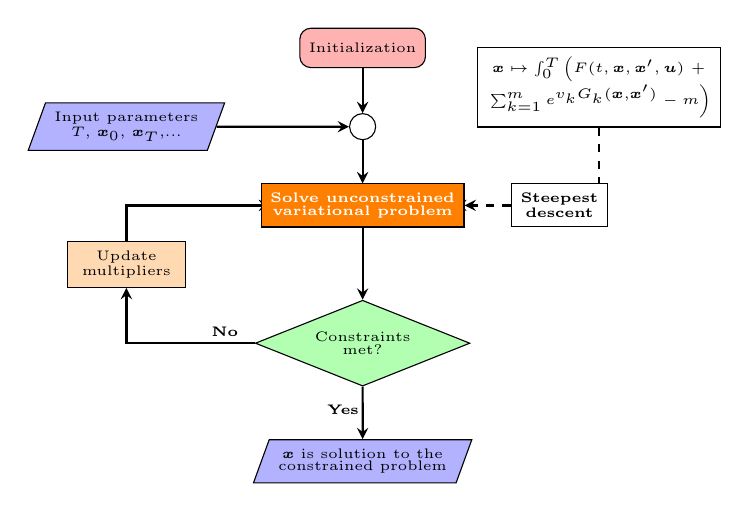
\begin{tikzpicture}[
		node distance=1cm, %Distance between nodes
		every text node part/.style={align=center}, %To allow multiline inside nodes
		execute at begin node=\setlength{\baselineskip}{.1em}
		]
		\onslide<1->{}
		
		\onslide<2->{
			\node (init) [startstop] {\tiny Initialization};
		}
		
		\onslide<3->{
			\node (point2) [point, below of=init] { };
			\node (input_params) [io ,left of=point2, xshift=-2cm] {\tiny Input parameters\\ \tiny $T$, $\bm{x}_0$, $\bm{x}_T$,...};
			\draw[arrow] (init) -- (point2);
			\draw[arrow] (input_params) -- (point2);
		}
		
		\onslide<4->{
			\node (uncr_minim) [process, below of=point2] {\tiny Solve unconstrained\\ \tiny variational problem};
			\draw[arrow] (point2) -- (uncr_minim);
		}
		
		\uncover<5>{
			\node (modif_problem) [whitebox, above of=uncr_minim, yshift=.5cm, xshift=3cm] {\tiny $\bm{x}\mapsto \int_0^T \left(F(t,\bm{x},\bm{x}',\bm{u}) \right. +$ \\ \tiny $\left.\sum_{k=1}^{m}e^{v_kG_k(\bm{x},\bm{x}')} - m \right)$};
			\draw [arrow-] (modif_problem) |- (uncr_minim);
		}
		
		\onslide<6->{
			\node (decision) [decision, below of=uncr_minim, yshift=-.75cm] {\tiny Constraints\\ \tiny met?};
			\draw[arrow] (uncr_minim) -- (decision);
		}
		
		\onslide<7->{
			\node [below of=decision, xshift=-.25cm, yshift=.15cm] {\tiny \textbf{Yes}};
		}
		
		\onslide<8->{
			\node (output) [io, below of=decision, yshift=-.50cm] {\tiny $\bm{x}$ is solution to the\\ \tiny constrained problem};
			\draw[arrow] (decision) -- (output);
		}
		
		\onslide<9->{
			\node [left of=decision, xshift=-.75cm, yshift=.15cm] {\tiny \textbf{No}};		
		}
		
		\onslide<10->{		
			\node (update) [process, left of=decision, xshift=-2cm, yshift=1cm] {\tiny Update\\ \tiny multipliers};
			\draw[arrow] (decision) -|  (update);
			
		}
		
		\onslide<11->{
			\draw[arrow] (update) |- (uncr_minim);
		}
		
		\onslide<12->{
			\node (uncr_minim2) [emphasis, below of=point2] {\tiny \textcolor{white}{\textbf{Solve unconstrained}}\\ \tiny \textcolor{white}{\textbf{variational problem}}};
			\node (steepest) [whitebox, right of=uncr_minim, xshift=1.5cm] {\tiny \textbf{Steepest}\\ \tiny \textbf{descent}};
			\draw[arrow-] (steepest) -- (uncr_minim2);
		}
		\end{tikzpicture}
	\end{figure}
\end{frame}

%\subsection{Unconstrained minimization}
%\begin{frame}[t] \frametitle{Unconstrained minimization \onslide<2->{\alert{(Steepest descent algorithm)}}}
%	\begin{figure}[width=\linewidth]
%		\centering
%		\begin{tikzpicture}[
%		node distance=1cm, %Distance between nodes
%		every text node part/.style={align=center}, %To allow multiline inside nodes
%		execute at begin node=\setlength{\baselineskip}{.1em}
%		]
%		
%		\onslide<2->{}
%		
%		\onslide<3->{
%			\node (init) [startstop] {\tiny Initialization}; 
%		}
%		
%		\onslide<4->{
%			\node (point1) [point, below of=init] { };
%			\draw [arrow] (init) -- (point1);
%			\node (input_params) [io, left of=point1, xshift=-2cm] {\tiny Input parameters \\ \tiny $T$, $\bm{x}_0$, $\bm{x}_T$,...};
%			\draw [arrow] (input_params) -- (point1);
%		}
%		
%		\onslide<5->{
%			\node (descent) [process, below of=point1] {\tiny Compute descent \\ \tiny direction $\bm{U}$};
%			\draw [arrow] (point1) -- (descent);
%		}
%		
%		\onslide<6->{
%			\node (norm_decision) [decision, below of=descent, yshift=-.75cm] {\tiny Is $||\bm{U}||$ small?};
%			\draw [arrow] (descent) -- (norm_decision);
%		}
%		
%		\onslide<7->{
%			\node [below of=norm_decision, xshift=-.25cm, yshift=.15cm] {\tiny \textbf{Yes}};
%		}
%		
%		\onslide<8->{
%			\node (output_x) [io, below of=norm_decision, yshift=-.5cm] {\tiny $\bm{x}$ is solution to the\\ \tiny unconstrained problem};
%			\draw [arrow] (norm_decision) -- (output_x);
%		}
%		
%		\onslide<9->{
%			\node [left of=norm_decision, xshift=-.75cm, yshift=.15cm] {\tiny \textbf{No}};
%		}
%		
%		\onslide<10->{
%			\node (step_size) [process, left of=norm_decision, xshift =-2cm] {\tiny Compute \\ \tiny step size $\tau$};
%			\draw [arrow] (norm_decision) -- (step_size);	
%		}
%		
%		\onslide<11->{
%			\node (update_x) [process, above of=step_size] {\tiny Update \tiny $\bm{x}\leftarrow\bm{x}+\tau\bm{U}$};
%			\draw [arrow] (step_size) -- (update_x);
%		}
%		
%		\onslide<12->{
%			\draw [arrow] (update_x) |- (descent);
%		}
%		\end{tikzpicture}
%		\label{fig:flowchart_unconstrained}
%	\end{figure}
%\end{frame}

\subsection{Algorithm for the solution of the LQR}
\begin{frame}[t] \frametitle{Algorithm for the solution of the LQR}
	\begin{figure}
		\centering
		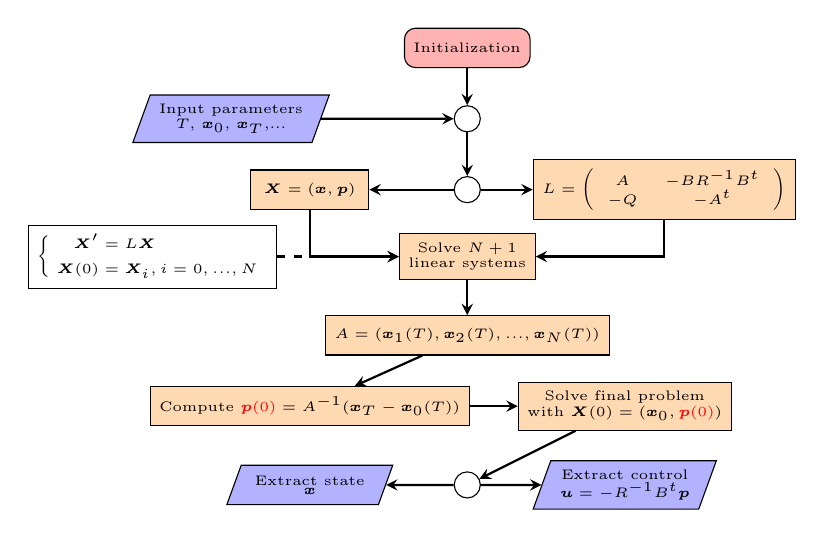
\begin{tikzpicture}[
		node distance=1cm, %Distance between nodes
		every text node part/.style={align=center}, %To allow multiline inside nodes
		execute at begin node=\setlength{\baselineskip}{.1em}
		]
		
		\onslide<1->{}
		
		\onslide<2->{
			\node (init) [startstop] {\tiny Initialization};
		}
		
		\onslide<3->{
			\node (point) [point, below of=init, yshift=.1cm] { };
			\node (input_params) [io, left of=point, xshift=-2cm] {\tiny Input parameters\\ \tiny $T$, $\bm{x}_0$, $\bm{x}_T$,...};
			\draw [arrow] (init) -- (point);
			\draw [arrow] (input_params) -- (point);
		}
		
		\onslide<4->{
			\node (point2) [point, below of=point, yshift=.1cm] {};
			\node (append) [process, left of=point2, xshift=-1cm] {\tiny $\bm{X} = \left(\bm{x},\bm{p}\right)$};
			\draw [arrow] (point) -- (point2);
			\draw [arrow] (point2) -- (append);
		}
		
		\onslide<5->{
			\node (matrix) [process, right of=point2, xshift=1.5cm] {\tiny $L = \left(\begin{array}{c c} A & -B R^{-1} B^t\\ -Q & -A^t \end{array} \right)$};
			\draw [arrow] (point2) -- (matrix);
		}
		
		\onslide<6->{
			\node (n_problems) [process, below of=matrix, xshift=-2.5cm, yshift=.15cm] {\tiny Solve $N+1$\\ \tiny linear systems};
			\draw [arrow] (append) |- (n_problems);
			\draw [arrow] (matrix) |- (n_problems);

		}
		\onslide<7>{
			\node (n_problems2) [whitebox, left of=n_problems, xshift=-3cm] {\tiny $\left\lbrace\begin{aligned} \bm{X}' &= L \bm{X}\\ \bm{X}(0) &= \bm{X}_i, i=0,...,N \end{aligned}\right. $ };
			\draw [arrow-] (n_problems2) -- (n_problems);		
		}
		\onslide<8->{
			\node (matrixA) [process, below of=n_problems] {\tiny $A = (\bm{x}_1(T),\bm{x}_2(T),...,\bm{x}_N(T))$};
			\draw [arrow] (n_problems) -- (matrixA);
		}
		
		\onslide<9->{
			\node (costate) [process, below of=matrixA, xshift=-2cm, yshift=.1cm] {\tiny Compute $\bm{p}(0) = A^{-1}(\bm{x}_T - \bm{x}_0(T))$};
			\draw [arrow] (matrixA) -- (costate);
		}
		
		\onslide<10->{
			\node (final) [process, below of=matrixA, xshift=2cm, yshift=.1cm] {\tiny Solve final problem\\ \tiny with $\bm{X}(0) = \left(\bm{x}_0,\bm{p}(0) \right)$ };
			\draw [arrow] (costate) -- (final);
		}
		
		\onslide<11->{	
			\node [process, below of=matrixA, xshift=-2cm, yshift=.1cm] {\tiny Compute $\textcolor{red}{\bm{p}(0)} = A^{-1}(\bm{x}_T - \bm{x}_0(T))$};
			\node [process, below of=matrixA, xshift=2cm, yshift=.1cm] {\tiny Solve final problem\\ \tiny with $\bm{X}(0) = \left(\bm{x}_0, \textcolor{red}{\bm{p}(0)}\right)$ };
		}
		
		\onslide<12->{
			\node (point3) [point, below of=final, xshift=-2cm] { };
			\node (state) [io, left of=point3, xshift=-1cm] {\tiny Extract state\\ \tiny $\bm{x}$};
			\draw [arrow] (final) -- (point3);
			\draw [arrow] (point3) -- (state);	
		}
		
		\onslide<13->{	
			\node (control) [io, right of=point3, xshift=1cm] {\tiny Extract control\\ \tiny $\bm{u} = -R^{-1}B^{t}\bm{p}$ };
			\draw [arrow] (point3) -- (control);
		}
		\end{tikzpicture}
	\end{figure}
\end{frame}

\section{Results}
\begin{frame}
	\sectionpage
\end{frame}

\begin{frame}
	\pause
	All simulations were performed with a functional of the type
	\pause
	\begin{block}{Functional}
		$$\bm{u}\longmapsto \dfrac{1}{2}\int_0^T \bm{x}^tQ\bm{x} + \bm{u}^tR\bm{u}$$
	\end{block}
\end{frame}

\subsection{\textbf{Linearised model} -- detumbling}
\begin{frame}[t] \frametitle{Linearised model \onslide<2->{ -- Detumbling}}
	\begin{columns}
		\column[t]{.55\linewidth}
		\onslide<3->{
			\begin{itemize}
				\item Objective:
				\begin{itemize}
					\item Dissipate rotational energy.
				\end{itemize}
				\item Initial state:
				\begin{itemize}
					\item Tumbling ($\bm{\omega} \neq \bm{0}$).
					\item $\text{(pitch,roll,yaw)} = (0,0,0)rad$.
				\end{itemize}
				\item Final state:
				\begin{itemize}
					\item At rest ($\bm{\omega} = \bm{0}$).
					\item $\text{(pitch,roll,yaw)} = (0,0,0)rad$.
				\end{itemize}
			\end{itemize}
		}
		\column[t]{.45\linewidth}
		\only<4>{
			\begin{figure}
				\centering
				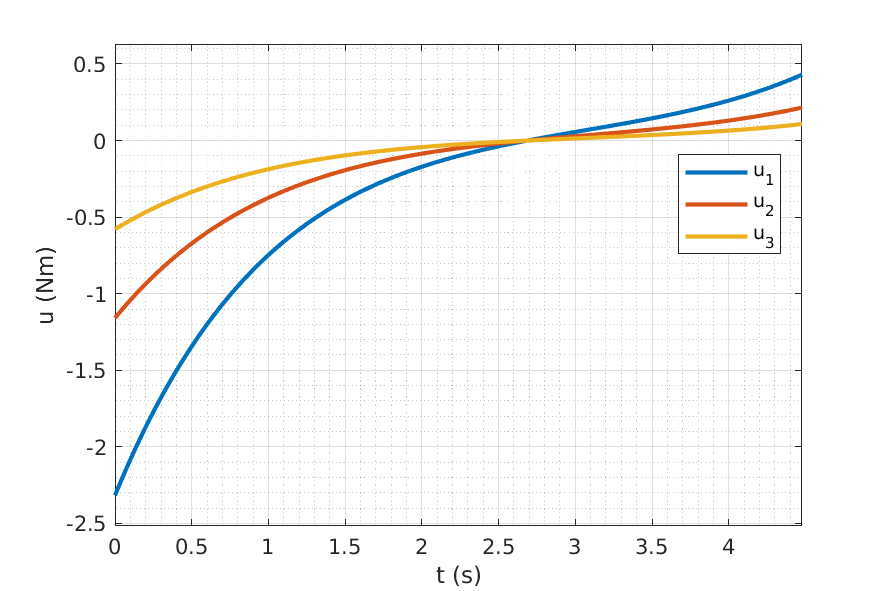
\includegraphics[width=1\linewidth]{./results/detumbling_fixed_j1_linear/figures_control}
				\caption{Control}
			\end{figure}
		}
		\only<5>{
			\begin{figure}
				\centering
				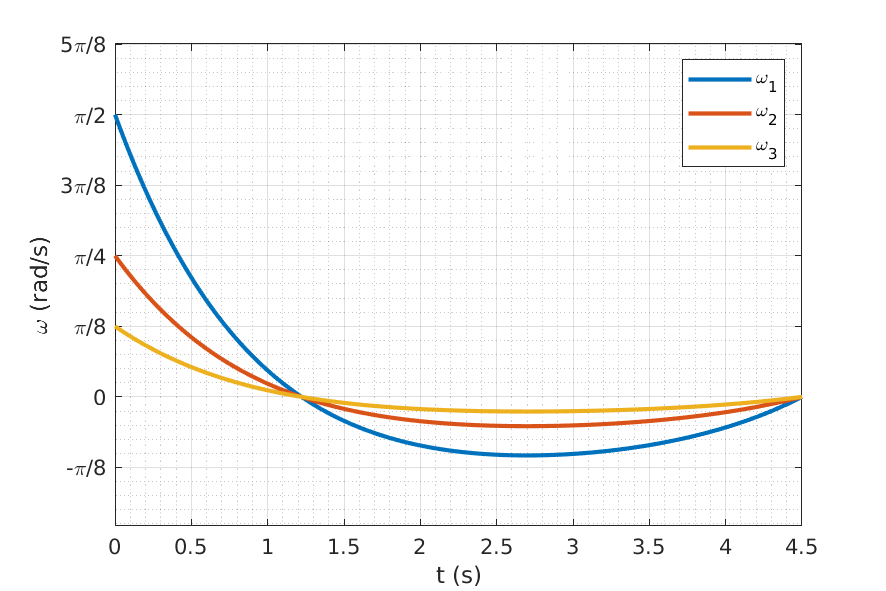
\includegraphics[width=1\linewidth]{./results/detumbling_fixed_j1_linear/figures_angveloc}
				\caption{Angular velocities}
			\end{figure}
		}
		\only<6>{
			\begin{figure}
				\centering
				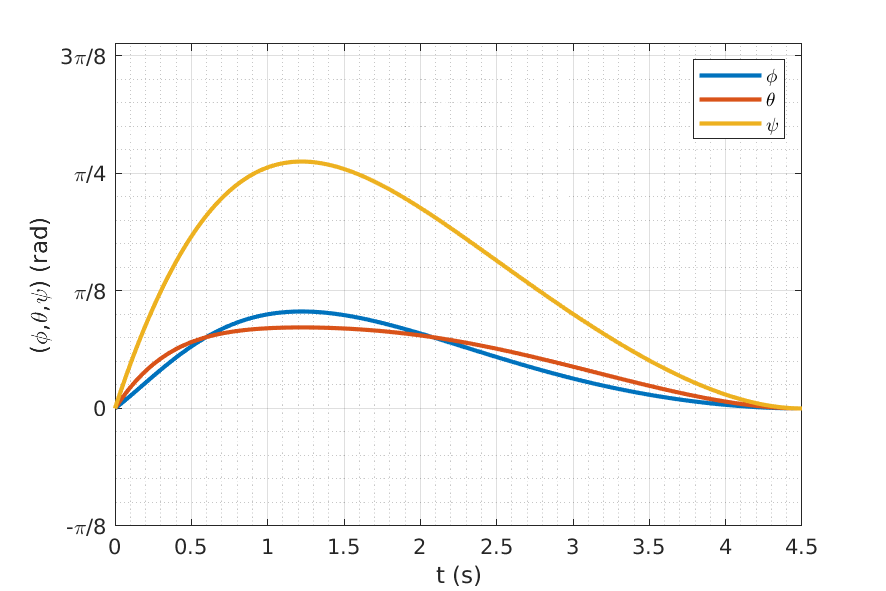
\includegraphics[width=1\linewidth]{./results/detumbling_fixed_j1_linear/figures_eulerang}
				\caption{Euler angles}
			\end{figure}
		}
	\end{columns}
\end{frame}

\begin{frame} \frametitle{Simulation parameters}
	{\tiny
		\begin{table}
			\centering
			\begin{tabular}{cccc}
				\toprule
				\textbf{Name} & \textbf{Symbol} & \textbf{Value} & \textbf{Unit} \\
				\midrule
				Final time & $T$ & $4.5$ & $s$ \\
				Tensor of inertia & $J$ & $I_3$ & $kg\ m^2$ \\
				\multirow{2}{*}{ Integrand\ \
					$F = \frac{1}{2}( \bm{x}^tQ\bm{x} + \bm{u}^tR\bm{u})$ } & $Q$ & $I_6$ & \\
				& $R$ & $I_3$ & \\
				Initial angular velocity & $\bm{\omega}_0$ & $(\pi/2,\pi/4,\pi/8)$ & $rad/s$ \\
				Final angular velocity & $\bm{\omega}_T$ & $(0,0,0)$ & $rad/s$ \\
				Initial orientation (Euler angles) & $\Phi_0$ & $(0,0,0)$ & $rad$ \\
				Final orientation (Euler angles) & $\Phi_T$ & $(0,0,0)$ & $rad$ \\
				\bottomrule
			\end{tabular}
			\caption{Simulation parameters}
		\end{table}
	}
\end{frame}

\begin{frame} \frametitle{Simulation results}
	\tiny{
		\only<+>{
			\begin{table}
				\centering
				\begin{tabular}{cccc}
					\toprule 
					\textbf{Name} & \textbf{Symbol} & \textbf{Value} & \textbf{Unit} \\
					\midrule
					Achieved final angular velocity & $\bm{\omega}(T)$ & $(4.22,2.11,2.14)10^{-3}$ & $rad/s$ \\
					Error in final angular velocity & $|\bm{\omega}(T)-\bm{\omega}_T|$ & $8.39\cdot 10^{-3}$ & $rad/s$\\
					Achieved final orientation & $\Phi(T)$ & $(8.48,1.63,3.29)10^{-3}$ & $rad$ \\
					Error in final orientation & $|\Phi(T)-\Phi_T|$ & $3.77\cdot 10^{-2}$ & $rad$ \\
					Cost & $I(\bm{u})$ & $4.95$ & \\
					CPU time & & $1.68\cdot 10^{-3}$ & s \\
					\bottomrule
				\end{tabular}
				\caption{Simulation results}
			\end{table}
		}
		\only<+>{
			\begin{table}
				\centering
				\begin{tabular}{cccc}
					\toprule 
					\textbf{Name} & \textbf{Symbol} & \textbf{Value} & \textbf{Unit} \\
					\midrule
					Achieved final angular velocity & $\bm{\omega}(T)$ & $(4.22,2.11,2.14)10^{-3}$ & $rad/s$ \\
					\rowcolor{yellow}
					Error in final angular velocity & $|\bm{\omega}(T)-\bm{\omega}_T|$ & $8.39\cdot 10^{-3}$ & $rad/s$\\
					Achieved final orientation & $\Phi(T)$ & $(8.48,1.63,3.29)10^{-3}$ & $rad$ \\
					\rowcolor{yellow}
					Error in final orientation & $|\Phi(T)-\Phi_T|$ & $3.77\cdot 10^{-2}$ & $rad$ \\
					Cost & $I(\bm{u})$ & $4.95$ & \\
					CPU time & & $1.68\cdot 10^{-3}$ & s \\
					\bottomrule
				\end{tabular}
				\caption{Simulation results}
			\end{table}
		}
	}
\end{frame}

\begin{frame} \frametitle{Simulation parameters}
	{\tiny
		\only<1>{
			\begin{table}
				\centering
				\begin{tabular}{cccc}
					\toprule
					\textbf{Name} & \textbf{Symbol} & \textbf{Value} & \textbf{Unit} \\
					\midrule
					Final time & $T$ & $4.5$ & $s$ \\
					Tensor of inertia & $J$ & $I_3$ & $kg\ m^2$ \\
					\multirow{2}{*}{ Integrand\ \
						$F = \frac{1}{2}( \bm{x}^tQ\bm{x} + \bm{u}^tR\bm{u})$ } & $Q$ & $I_6$ & \\
					& $R$ & $I_3$ & \\
					Initial angular velocity & $\bm{\omega}_0$ & $(\pi/2,\pi/4,\pi/8)$ & $rad/s$ \\
					Final angular velocity & $\bm{\omega}_T$ & $(0,0,0)$ & $rad/s$ \\
					Initial orientation (Euler angles) & $\Phi_0$ & $(0,0,0)$ & $rad$ \\
					Final orientation (Euler angles) & $\Phi_T$ & $(0,0,0)$ & $rad$ \\
					\bottomrule
				\end{tabular}
				\caption{Simulation parameters.}
			\end{table}	
		}
		\only<2>{
			\begin{table}
				\centering
				\begin{tabular}{cccc}
					\toprule
					\textbf{Name} & \textbf{Symbol} & \textbf{Value} & \textbf{Unit} \\
					\midrule
					Final time & $T$ & $4.5$ & $s$ \\
					\rowcolor{yellow}
					Tensor of inertia & $J$ & $I_3$ & $kg\ m^2$ \\
					\multirow{2}{*}{ Integrand\ \
						$F = \frac{1}{2}( \bm{x}^tQ\bm{x} + \bm{u}^tR\bm{u})$ } & $Q$ & $I_6$ & \\
					& $R$ & $I_3$ & \\
					Initial angular velocity & $\bm{\omega}_0$ & $(\pi/2,\pi/4,\pi/8)$ & $rad/s$ \\
					Final angular velocity & $\bm{\omega}_T$ & $(0,0,0)$ & $rad/s$ \\
					Initial orientation (Euler angles) & $\Phi_0$ & $(0,0,0)$ & $rad$ \\
					Final orientation (Euler angles) & $\Phi_T$ & $(0,0,0)$ & $rad$ \\
					\bottomrule
				\end{tabular}
				\caption{Simulation parameters.}
			\end{table}
		}
	}
\end{frame}

\begin{frame} \frametitle{}
	\onslide<+->{Tensor of inertia $J$} \onslide<+->{proportional to the identity} \onslide<+->{$\Rightarrow$} \onslide<+->{$\bm{\omega}\times J\bm{\omega} = \bm{0}$}
	\uncover<+->{
		\begin{equation*}
		\left\lbrace\begin{array}{c}
		\begin{aligned}
		J \bm{\omega}' & = -\textcolor{red}{\cancel{\bm{\omega}\times J\bm{\omega}}} + \bm{u} \\
		\bm{\epsilon}' & = -\dfrac{1}{2}\bm{\omega}\times\bm{\epsilon} + \dfrac{1}{2}\eta\bm{\omega} \\
		\eta' & = - \dfrac{1}{2}\bm{\omega}^t\bm{\epsilon}
		\end{aligned}
		\end{array}\right.
		\end{equation*}
	}
	\onslide<+->{ Nonlinear effects are less noticeable.}
\end{frame}

\begin{frame} \frametitle{If $J$ is not proportional to the identity}
	\begin{columns}
		\column{.5\linewidth}
		\onslide<2->{
			Identical configuration, except:
			$$
			J = \left(\begin{array}{ccc}
			1 & 0 & 0 \\
			0 & 0.75 & 0 \\
			0 & 0 & 0.5 
			\end{array}\right)
			kg\ m^2
			$$
		}
		\column{.5\linewidth}
		\only<3>{
			\begin{figure}
				\centering
				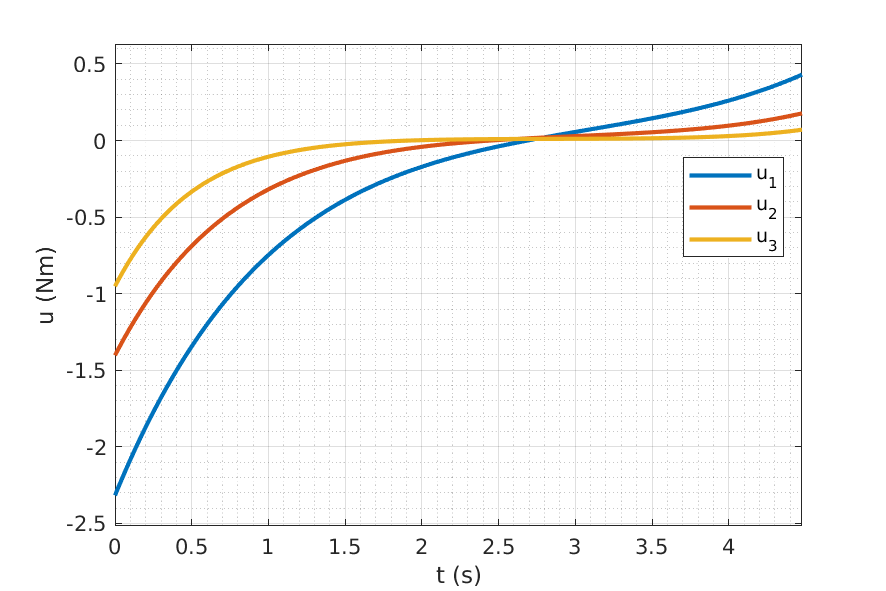
\includegraphics[width=1\linewidth]{./results/detumbling_fixed_linear_jnd/figures_control}
				\caption{Control}
			\end{figure}
		}
		\only<4>{
			\begin{figure}
				\centering
				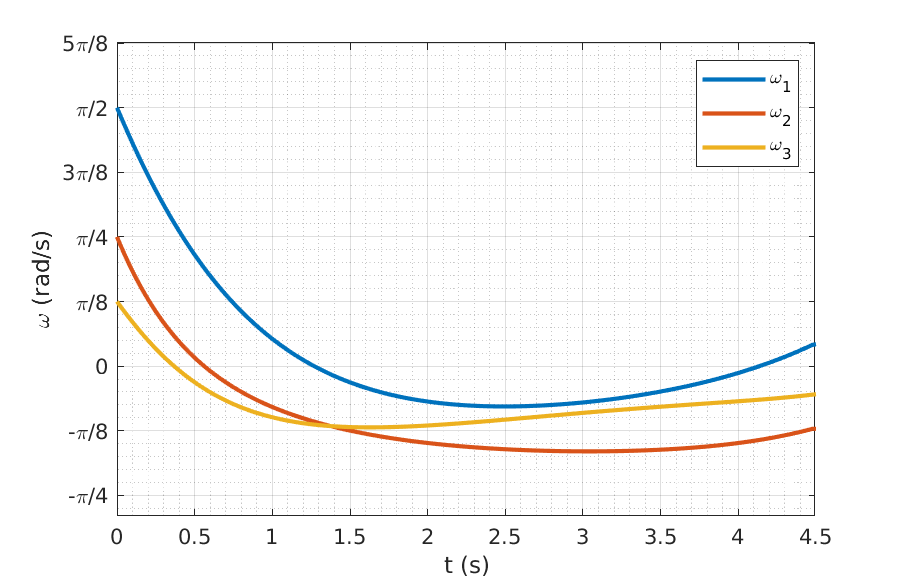
\includegraphics[width=1\linewidth]{./results/detumbling_fixed_linear_jnd/figures_real_angveloc}
				\caption{Angular velocities}
			\end{figure}
		}
		\only<5>{
			\begin{figure}
				\centering
				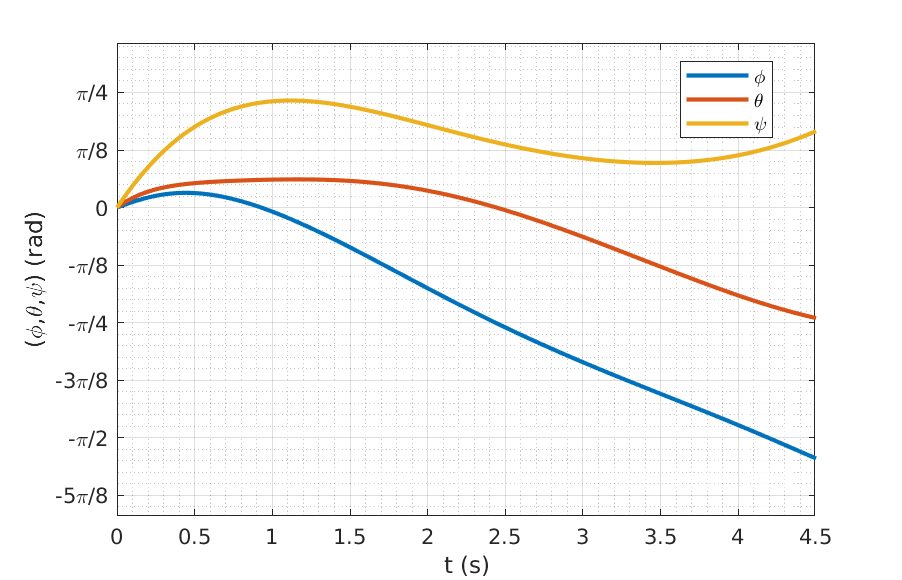
\includegraphics[width=1\linewidth]{./results/detumbling_fixed_linear_jnd/figures_real_eulerang}
				\caption{Euler angles}
			\end{figure}
		}
	\end{columns}
\end{frame}

\begin{frame} \frametitle{If $J$ is not proportional to the identity -- Simulation results}
	\tiny{
		\only<+>{
			\begin{table}
				\centering
				\begin{tabular}{cccc}
					\toprule 
					\textbf{Name} & \textbf{Symbol} & \textbf{Value} & \textbf{Unit} \\
					\midrule
					Achieved final angular velocity & $\bm{\omega}(T)$ & $(1.33,-3.81,-1.71)10^{-1}$ & $rad/s$ \\
					Error in final angular velocity & $|\bm{\omega}(T)-\bm{\omega}_T|$ & $4.38\cdot 10^{-1}$ & $rad/s$\\
					Achieved final orientation & $\Phi(T)$ & $(-1.71,-0.75,0.52)$ & $rad$ \\
					Error in final orientation & $|\Phi(T)-\Phi_T|$ & $1.94$ & $rad$ \\
					Cost & $I(\bm{u})$ & $4.52$ & \\
					CPU time & & $2.56\cdot 10^{-3}$ & s \\
					\bottomrule
				\end{tabular}
				\caption{Simulation results.}
			\end{table}
		}
		\only<+>{
			\begin{table}
				\centering
				\begin{tabular}{cccc}
					\toprule 
					\textbf{Name} & \textbf{Symbol} & \textbf{Value} & \textbf{Unit} \\
					\midrule
					Achieved final angular velocity & $\bm{\omega}(T)$ & $(1.33,-3.81,-1.71)10^{-1}$ & $rad/s$ \\
					\rowcolor{yellow}
					Error in final angular velocity & $|\bm{\omega}(T)-\bm{\omega}_T|$ & $4.38\cdot 10^{-1}$ & $rad/s$\\
					Achieved final orientation & $\Phi(T)$ & $(-1.71,-0.75,0.52)$ & $rad$ \\
					\rowcolor{yellow}
					Error in final orientation & $|\Phi(T)-\Phi_T|$ & $1.94$ & $rad$ \\
					Cost & $I(\bm{u})$ & $4.52$ & \\
					CPU time & & $2.56\cdot 10^{-3}$ & s \\
					\bottomrule
				\end{tabular}
				\caption{Simulation results.}
			\end{table}
		}
	}	
\end{frame}

\begin{frame} \frametitle{If $J$ is not proportional to the identity -- Simulation results}
	\only<1>{
	\begin{itemize}
		\item Error in angular velocity:
		\begin{itemize}
			\item[] \begin{center} $|\bm{\omega}(T)-\bm{\omega}_T| = 0.44\ rad/s$ $\approx  4\ rpm$ \end{center}
		\end{itemize}
		\item Error in orientation (Euler angles):
		\begin{itemize}
			\item[] \begin{center} $|\phi(T)-\phi_T| = 1.94\ rad$ $\approx  \alert{1 11^\circ}$ \end{center}
		\end{itemize} 
	\end{itemize}
	}
	\only<2>{The linearised model \alert{is not able} to steer the system to the desired state.}
\end{frame}

\subsection{\textbf{Nonlinear model} -- detumbling}
\begin{frame} \frametitle{Nonlinear model \onslide<2->{ -- Detumbling}}
	\onslide<3->{
		\begin{itemize}
			\item Objective:
			\begin{itemize}
				\item Dissipate rotational energy.
			\end{itemize}
			\item Initial state:
			\begin{itemize}
				\item Tumbling ($\bm{\omega} \neq \bm{0}$).
				\item $\text{(pitch,roll,yaw)} = (0,0,0)rad$.
			\end{itemize}
			\item Final state:
			\begin{itemize}
				\item At rest ($\bm{\omega} = \bm{0}$).
				\item $\text{(pitch,roll,yaw)} = (0,0,0)rad$.
			\end{itemize}
		\end{itemize}
	}				
\end{frame}

\begin{frame} \frametitle{Simulation parameters}
	\pause
	Parameters are set as in the previous case:
	\pause
	{\tiny
		\begin{table}
			\centering
			\begin{tabular}{cccc}
				\toprule
				\textbf{Name} & \textbf{Symbol} & \textbf{Value} & \textbf{Unit} \\
				\midrule
				Final time & $T$ & $4.5$ & $s$ \\
				\multirow{2}{*}{ Integrand\ \
					$F = \frac{1}{2}( \bm{x}^tQ\bm{x} + \bm{u}^tR\bm{u})$ } & $Q$ & $I_7$ & \\
				& $R$ & $I_3$ & \\
				Initial angular velocity & $\bm{\omega}_0$ & $(\pi/2,\pi/4,\pi/8)$ & $rad/s$ \\
				Final angular velocity & $\bm{\omega}_T$ & $(0,0,0)$ & $rad/s$ \\
				Initial orientation (Euler angles) & $\Phi_0$ & $(0,0,0)$ & $rad$ \\
				Final orientation (Euler angles) & $\Phi_T$ & $(0,0,0)$ & $rad$ \\
				\bottomrule
			\end{tabular}
			\caption{Simulation parameters}
		\end{table}
	}
\end{frame}

\begin{frame} \frametitle{Simulation results}
	\onslide<2> {The nonlinear model behaves well for any choice of $J$.}
\end{frame}

\begin{frame}[t] \frametitle{Simulation results}
	{\setlength{\baselineskip}{.1em}
		\begin{columns}
			\column[t]{.5\linewidth}
			\onslide<1->{\begin{center} $J = I_{3\times 3}$ \end{center}}
			\only<1>{
				\begin{figure}
					\centering
					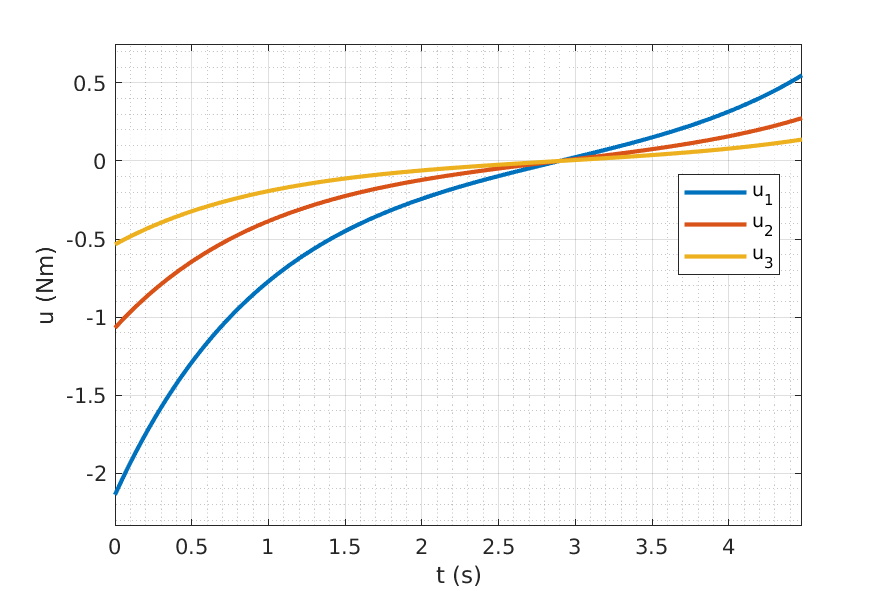
\includegraphics[width=\linewidth]{./results/detumbling_fixed_nonlinear_j1/figures_control}
					\caption{Control.}
				\end{figure}
			}
			\only<2>{
				\begin{figure}
					\centering
					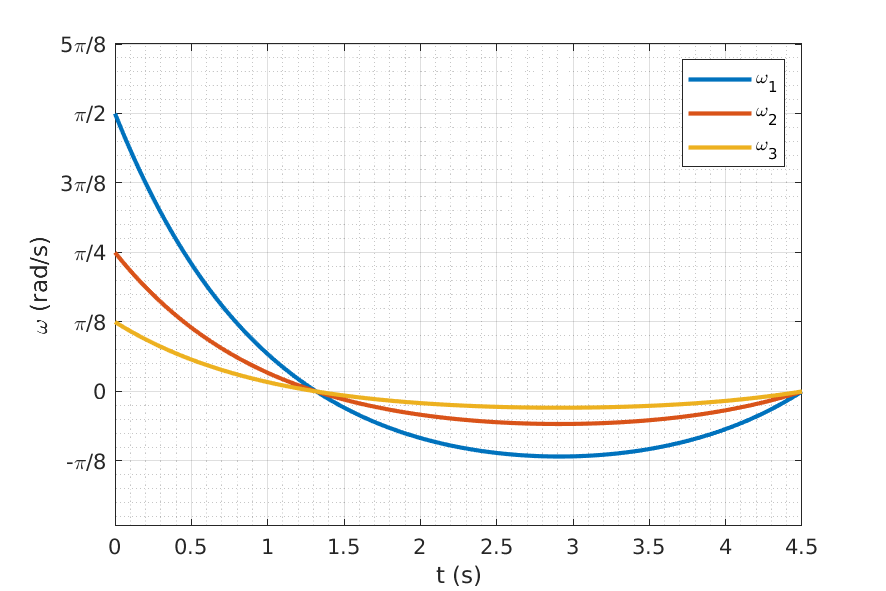
\includegraphics[width=\linewidth]{./results/detumbling_fixed_nonlinear_j1/figures_angveloc}
					\caption{Angular velocities.}
				\end{figure}
			}
			\only<3>{
				\begin{figure}
					\centering
					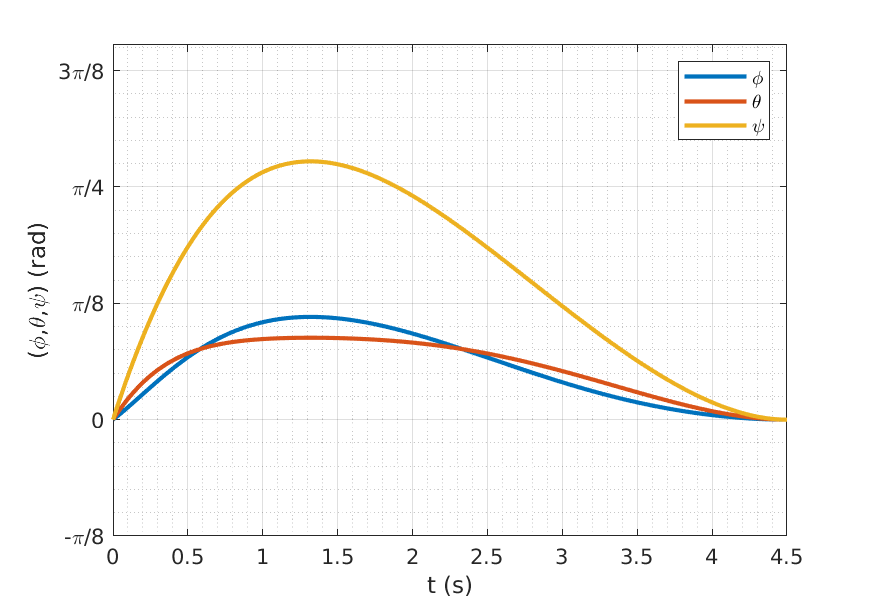
\includegraphics[width=\linewidth]{./results/detumbling_fixed_nonlinear_j1/figures_eulerang}
					\caption{Euler angles.}
				\end{figure}
			}
			\column[t]{.5\linewidth}
			\onslide<1->{\begin{center} $J = diag(1,0.75,0.5)$ \end{center}}
			\only<1>{
				\begin{figure}
					\centering
					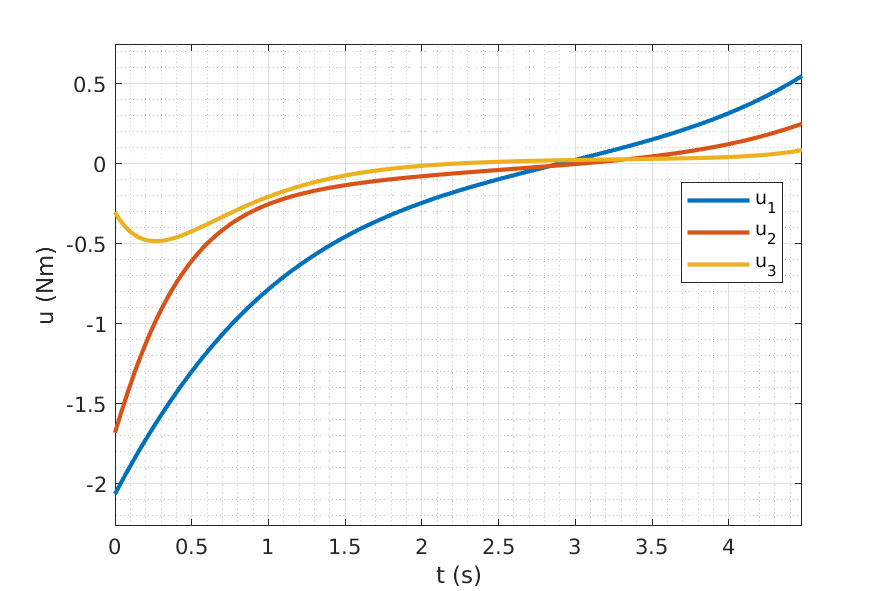
\includegraphics[width=\linewidth]{./results/detumbling_fixed_nonlinear_jnd/figures_control}
					\caption{Control.}
				\end{figure}
			}
			\only<2>{
				\begin{figure}
					\centering
					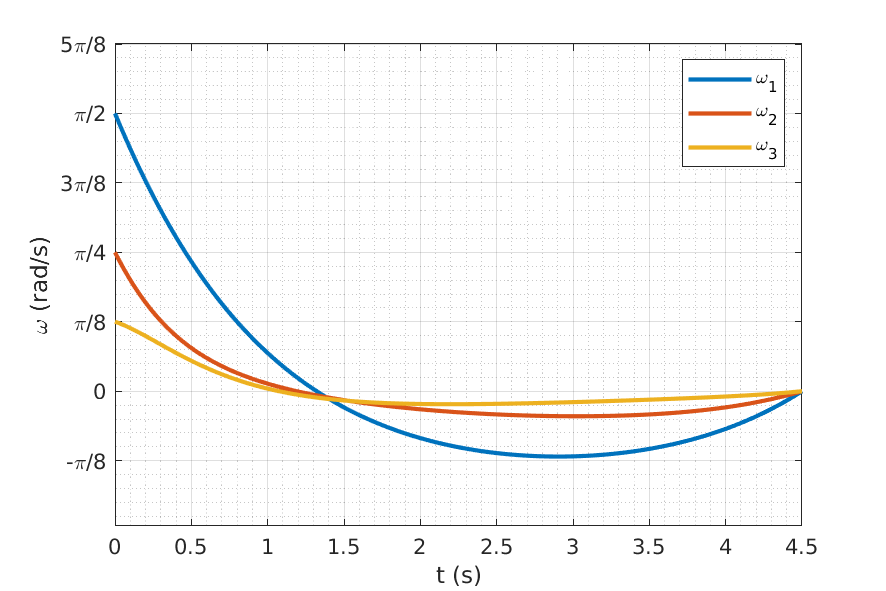
\includegraphics[width=\linewidth]{./results/detumbling_fixed_nonlinear_jnd/figures_angveloc}
					\caption{Angular velocities.}
				\end{figure}
			}
			\only<3>{
				\begin{figure}
					\centering
					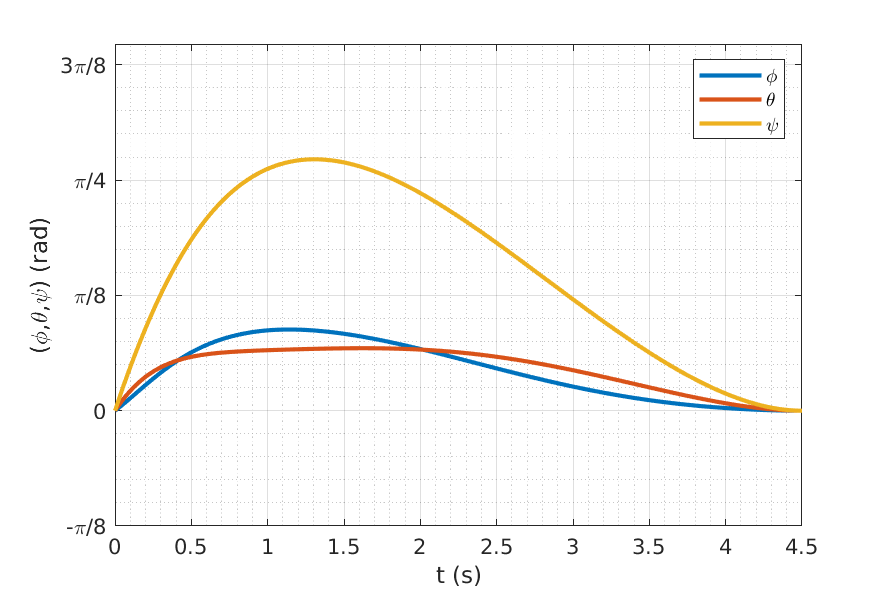
\includegraphics[width=\linewidth]{./results/detumbling_fixed_nonlinear_jnd/figures_eulerang}
					\caption{Euler angles}
				\end{figure}
			}
		\end{columns}
	}
\end{frame}

\begin{frame} \frametitle{J proportional to the identity -- Simulation results}
	\begin{itemize}
		\item Error in angular velocity:
		\begin{itemize}
			\item[] \begin{center} $|\bm{\omega}(T)-\bm{\omega}_T| = 7\cdot 10^{-3}\ rad/s$ $\approx  0.07\ rpm$ \end{center}
		\end{itemize}
		\item Error in orientation (Euler angles):
		\begin{itemize}
			\item[] \begin{center} $|\phi(T)-\phi_T| = 1.59\cdot 10^{-4}\ rad$ $\approx  0.009^\circ$ \end{center}
		\end{itemize}
	\end{itemize}
\end{frame}

\begin{frame} \frametitle{J not proportional to the identity -- Simulation results}
	\begin{itemize}
		\item Error in angular velocity:
		\begin{itemize}
			\item[] \begin{center} $|\bm{\omega}(T)-\bm{\omega}_T| = 6.1\cdot 10^{-3}\ rad/s$ $\approx  0.06\ rpm$ \end{center}
		\end{itemize}
		\item Error in orientation (Euler angles):
		\begin{itemize}
			\item[] \begin{center} $|\phi(T)-\phi_T| = 1.55\cdot 10^{-4}\ rad$ $\approx  0.009^\circ$ \end{center}
		\end{itemize}
	\end{itemize}
\end{frame}

\begin{frame} \frametitle{J not proportional to the identity -- Simulation results}
	The nonlinear model \alert{is able} to steer the system to the desired state.
\end{frame}

\subsection{\textbf{Nonlinear model} -- single axis, rest to rest}
\begin{frame}[t] \frametitle{Nonlinear model \onslide<2->{ -- Single axis, rest to rest}}
	\begin{columns}
		\column[t]{.55\linewidth}
		\onslide<3->{
			\begin{itemize}
				\item Objective:
				\begin{itemize}
					\item Rotate $\pi/2\ rad$ around the $z$ axis.
				\end{itemize}
				\item Initial state:
				\begin{itemize}
					\item At rest ($\bm{\omega} = \bm{0}$).
					\item $\text{(pitch,roll,yaw)} = (0,0,0)rad$.
				\end{itemize}
				\item Final state:
				\begin{itemize}
					\item At rest ($\bm{\omega} = \bm{0}$).
					\item $\text{(pitch,roll,yaw)} = (\pi/2,0,0)rad$.
				\end{itemize}
				\item Inequality constraints on control: $|u_i|\leq 1Nm\ i=1,2,3.$
			\end{itemize}
		}
		\column[t]{.45\linewidth}
		\only<4>{
			\begin{figure}
				\centering
				\includegraphics[width=1\linewidth]{./results/sing_rest_rest_nonlinear_T2-515/figures_control}
				\caption{Control}
			\end{figure}
		}
		\only<5>{
			\begin{figure}
				\centering
				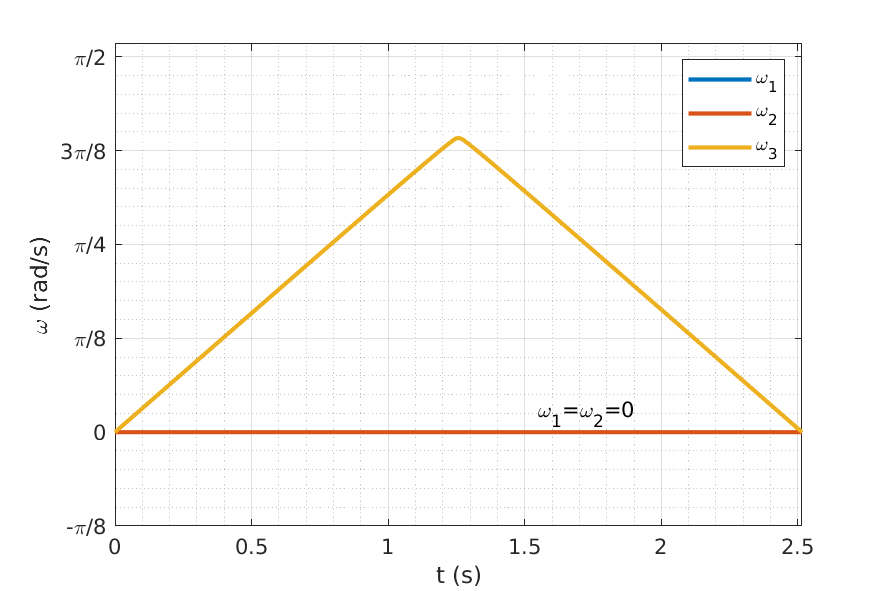
\includegraphics[width=1\linewidth]{./results/sing_rest_rest_nonlinear_T2-515/figures_angveloc}
				\caption{Angular velocities}
			\end{figure}
		}
		\only<6>{
			\begin{figure}
				\centering
				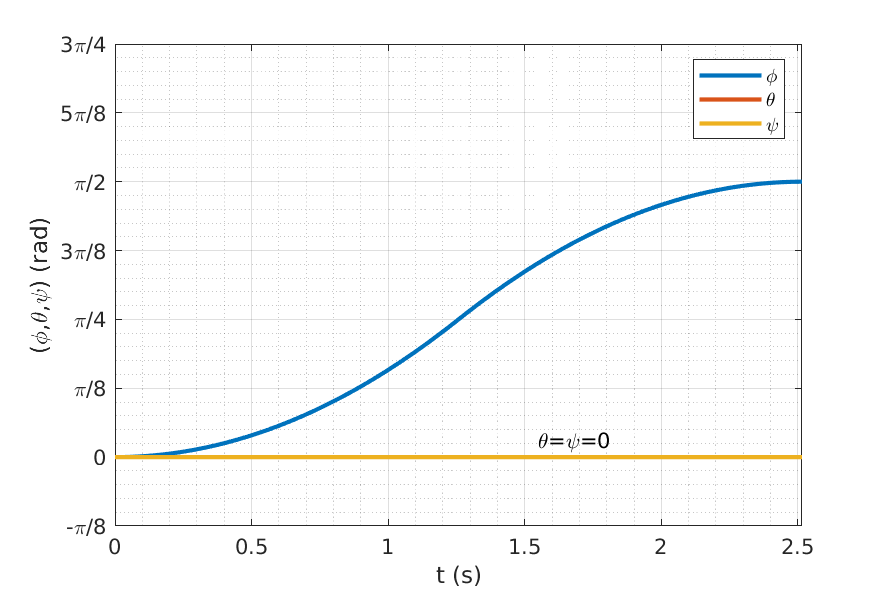
\includegraphics[width=1\linewidth]{./results/sing_rest_rest_nonlinear_T2-515/figures_eulerang}
				\caption{Euler angles}
			\end{figure}
		}
	\end{columns}
\end{frame}

\begin{frame} \frametitle{Simulation parameters}
	\pause
	{\tiny
		\begin{table}
			\centering
			\begin{tabular}{cccc}
				\toprule
				\textbf{Name} & \textbf{Symbol} & \textbf{Value} & \textbf{Unit} \\
				\midrule
				Final time & $T$ & $2.55, 2.525, 2.52$ & $s$ \\
				Tensor of inertia & $J$ & $diag(0.5, 0.75, 1)$ & $Kg\ m^2$ \\
				\multirow{2}{*}{ Integrand\ \
					$F = \frac{1}{2}( \bm{x}^tQ\bm{x} + \bm{u}^tR\bm{u})$ } & $Q$ & $0_6$ & \\
				& $R$ & $0_3$ & \\
				Initial angular velocity & $\bm{\omega}_0$ & $(0,0,0)$ & $rad/s$ \\
				Final angular velocity & $\bm{\omega}_T$ & $(0,0,0)$ & $rad/s$ \\
				Initial orientation (Euler angles) & $\Phi_0$ & $(0,0,0)$ & $rad$ \\
				Final orientation (Euler angles) & $\Phi_T$ & $(\pi/2,0,0)$ & $rad$ \\
				\bottomrule
			\end{tabular}
			\caption{Simulation parameters}
		\end{table}
	}
\end{frame}

\begin{frame} \frametitle{Bang-bang effect}
	\pause
	When inequality constraints on control are imposed
	\pause
	$$\text{For example: } |u_i| \leq 1\ Nm\ \ i=1,2,3$$
	\pause
	The control approaches a \textit{bang-bang} strategy as the time interval is reduced.	
\end{frame}

\begin{frame} \frametitle{Bang-bang effect}
	\only<1>{}
	\only<2>{
		\begin{figure}
			\centering
			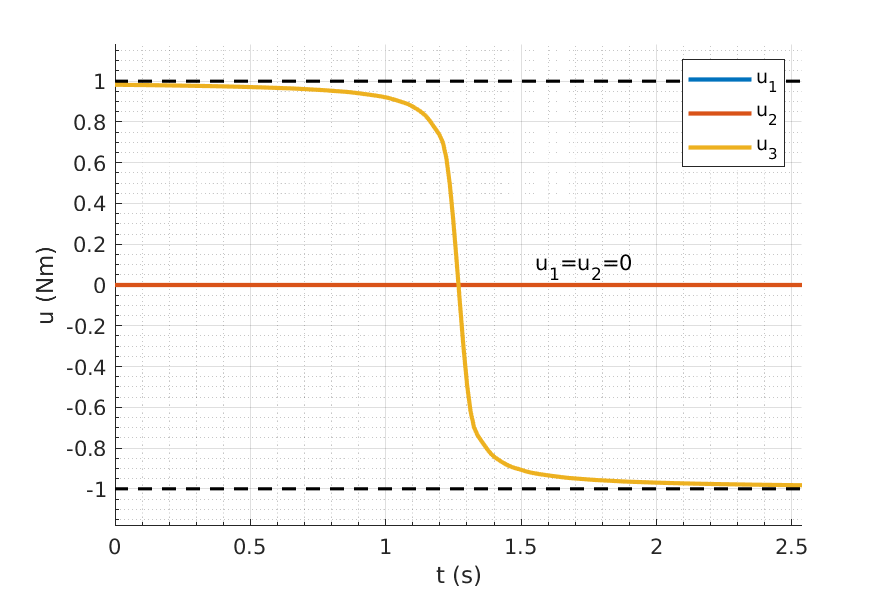
\includegraphics[width=.5\linewidth]{./results/sing_rest_rest_nonlinear_T2-55/figures_control}
			\caption{Control for $T=2.55s$.}
		\end{figure}
	}
	\only<3>{
		\begin{figure}
			\centering
			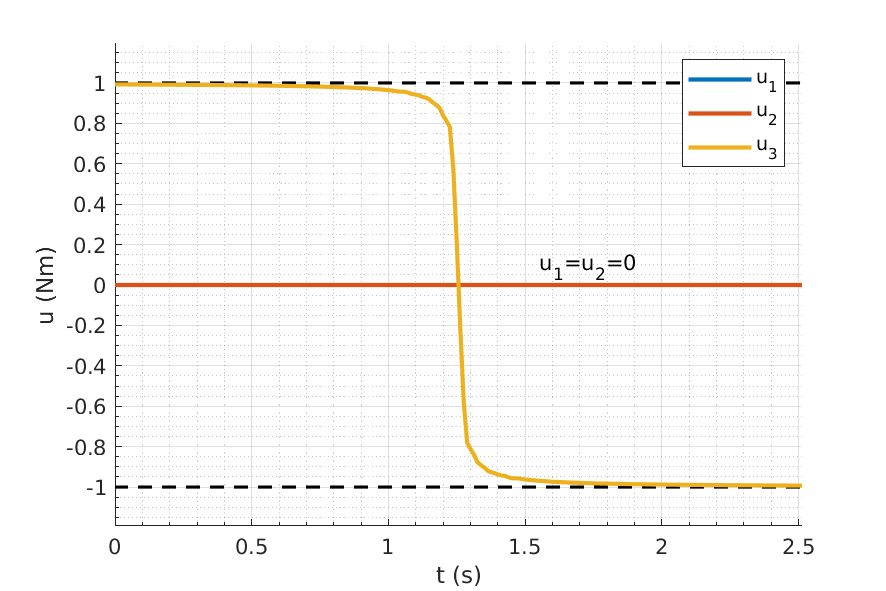
\includegraphics[width=.5\linewidth]{./results/sing_rest_rest_nonlinear_T2-525/figures_control}
			\caption{Control for $T=2.525s$.}
		\end{figure}
	}
	\only<4>{
		\begin{figure}
			\centering
			\includegraphics[width=.5\linewidth]{./results/sing_rest_rest_nonlinear_T2-52/figures_control}
			\caption{Control for $T=2.52s$.}
		\end{figure}
	}
\end{frame}

\begin{frame} \frametitle{Simulation results}
	\begin{itemize}
		\item Error in angular velocity:
		\begin{itemize}
			\item[] \begin{center} $|\bm{\omega}(T)-\bm{\omega}_T| = 2.84\cdot 10^{-3}\ rad/s$ $\approx  0.03\ rpm$ \end{center}
		\end{itemize}
		\item Error in orientation (Euler angles):
		\begin{itemize}
			\item[] \begin{center} $|\phi(T)-\phi_T| = 3.8\cdot 10^{-3}\ rad$ $\approx  0.2^\circ$ \end{center}
		\end{itemize}
	\end{itemize}
\end{frame}

\subsection{Animations}
\begin{center}
	\begin{frame} \frametitle{Animation -- Detumbling}
		\movie{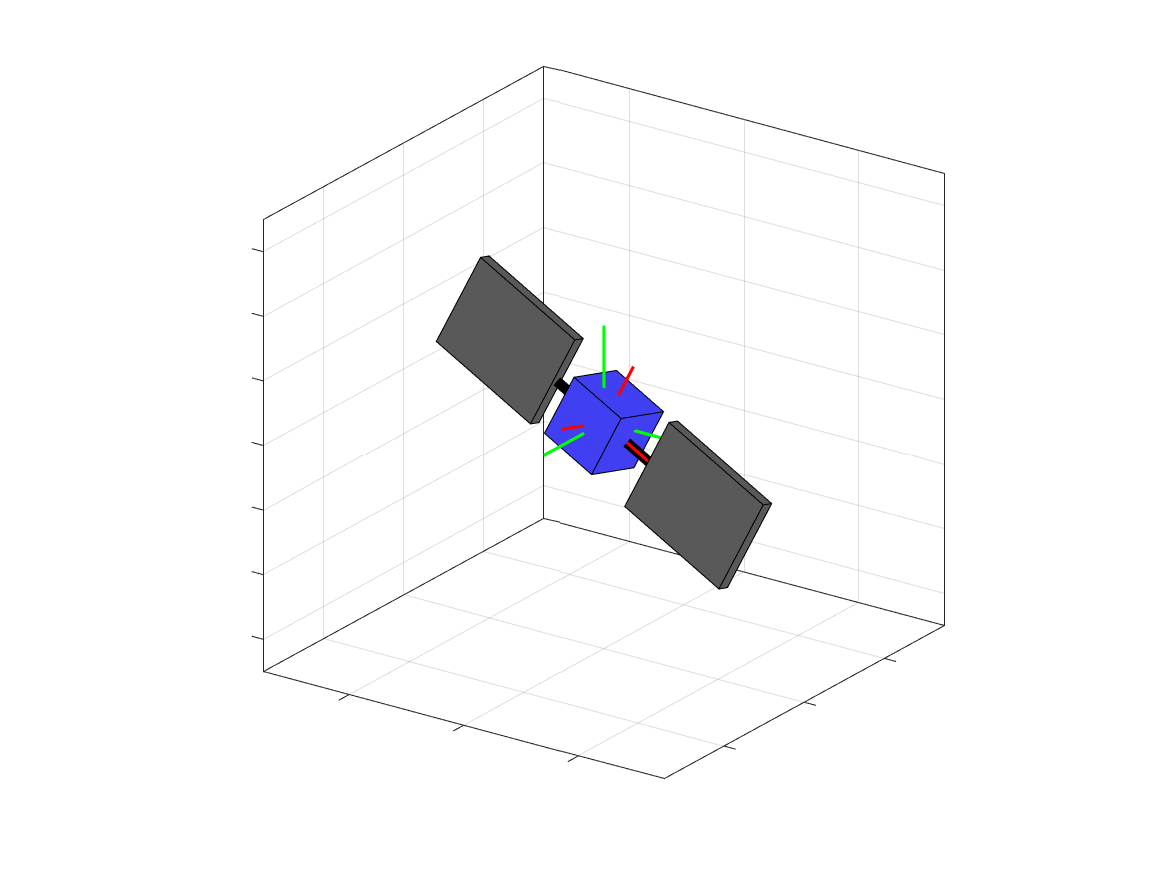
\includegraphics[width=.75\linewidth]{./animations/image_detumbling}}{./figures/animations/animation_detumbling.avi}
	\end{frame}
\end{center}

\begin{center}
	\begin{frame} \frametitle{Animation -- Single axis, rest to rest}
		\movie{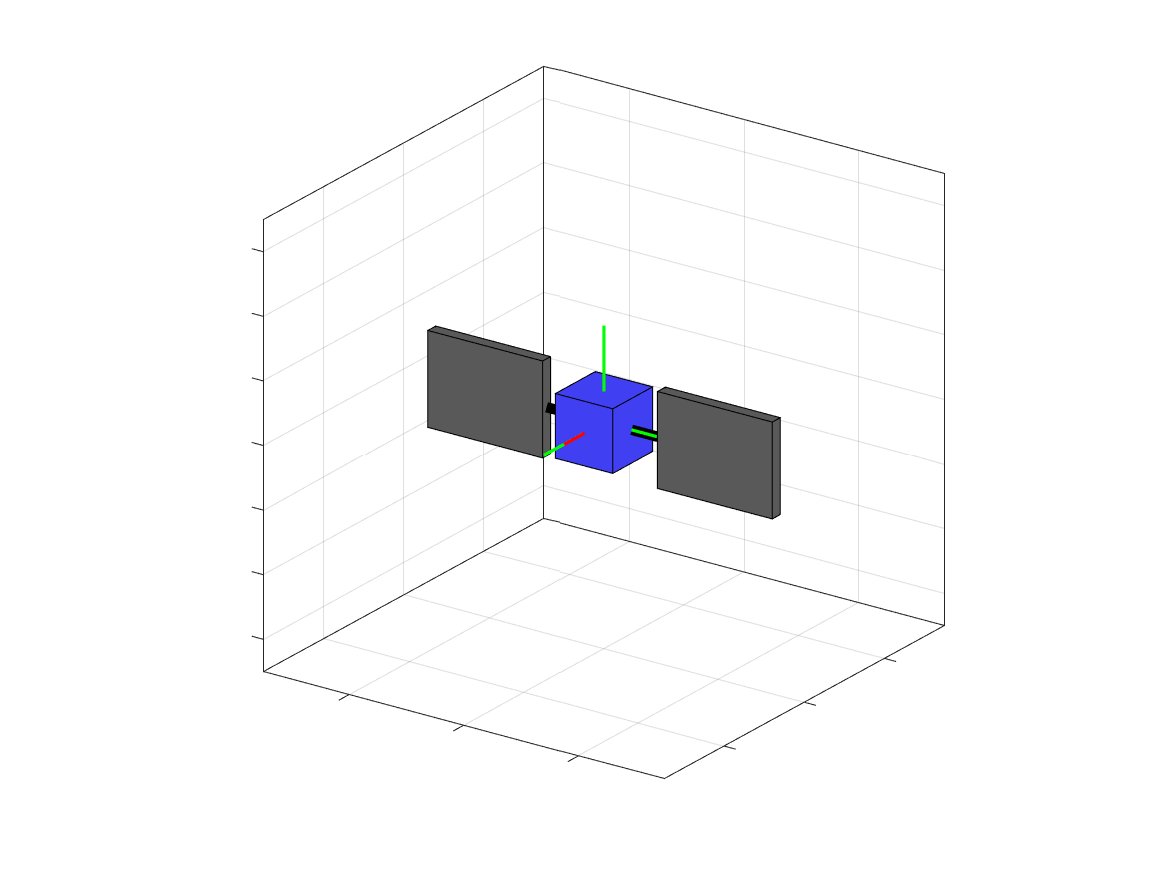
\includegraphics[width=.75\linewidth]{./animations/image_single_axis}}{./figures/animations/animation_single_axis.avi}
	\end{frame}
\end{center}


\section{Conclusions and future work}
\begin{frame}
	\sectionpage
\end{frame}

\subsection{Conclusions}
\begin{frame} \frametitle{Conclusions}
	\begin{itemize}
		\item<2-> Two different approaches have been employed:
		\begin{itemize}
			\item<3-> Linearised model.
			\item<4-> Nonlinear model (Main aim of the work).
		\end{itemize}
		\item<5-> Both have proven successful in certain situations.
	\end{itemize}
\end{frame}

\begin{frame}[t]{Comparison} %The t parameter aligns the text at the top
	\begin{columns}
		\column[t]{.5\linewidth} %The t parameter aligns the text at the top
		\begin{center} \textbf{Advantages of the nonlinear approach:} \end{center}
		\begin{itemize}
			\item<2-> Accuracy.
			\item<3-> Constraints.
			\item<4-> Larger class of integrands.
			\item<5-> Complex manoeuvres.
		\end{itemize}
		
		\column[t]{.5\linewidth} %The t parameter aligns the text at the top
		\begin{center} \textbf{Advantages of the linear approach:} \end{center}
		\begin{itemize} 
			\item<6-> Computation time.
			\begin{itemize}
				\item<7-> Linearised model: $CPU\ time \sim 10^{-3}s$.
				\item<7-> Nonlinear model: $CPU\ time \sim 10s$.
			\end{itemize}
		\end{itemize}
	\end{columns}
\end{frame}

\begin{frame}{Simulations} %The t parameter aligns the text at the top
	\begin{itemize}
		\item<2-> Fortran 95.
		\item<3-> Compiled with gfortran.
		\item<4-> Linux machine.
		\item<5-> Intel Core i7 4510U.
	\end{itemize}
\end{frame}

\subsection{Future work}
\begin{frame}{Future work}
	\begin{itemize}
		\item<2-> Controllability.
		\item<3-> Influence of:
		\begin{itemize}
			\item<4-> Magnetic actuation.
			\item<5-> Disturbances\onslide<6->{, such as atmospheric drag.}
		\end{itemize}
		\item<7-> Underactuated satellites.
		\item<8-> Uncertainty.
		\item<9-> Incomplete measurements.
		\item<10-> Improvement of numerical procedures.
		\item<11-> Implementation and testing.
	\end{itemize}
\end{frame}

\section*{}
\begin{frame}[c]{ }
	\onslide<2>{
	\begin{center}
		{\Huge Thank you.}
	\end{center}
	}
\end{frame}

\nobibliography{./bibliography/bibliography}
\bibliographystyle{apalike}

\end{document}